\documentclass[14pt]{extbook}
\usepackage{multicol, enumerate, enumitem, hyperref, color, soul, setspace, parskip, fancyhdr} %General Packages
\usepackage{amssymb, amsthm, amsmath, latexsym, units, mathtools} %Math Packages
\everymath{\displaystyle} %All math in Display Style
% Packages with additional options
\usepackage[headsep=0.5cm,headheight=12pt, left=1 in,right= 1 in,top= 1 in,bottom= 1 in]{geometry}
\usepackage[usenames,dvipsnames]{xcolor}
\usepackage{dashrule}  % Package to use the command below to create lines between items
\newcommand{\litem}[1]{\item#1\hspace*{-1cm}\rule{\textwidth}{0.4pt}}
\pagestyle{fancy}
\lhead{Progress Quiz 7}
\chead{}
\rhead{Version C}
\lfoot{3510-5252}
\cfoot{}
\rfoot{Summer C 2021}
\begin{document}

\begin{enumerate}
\litem{
Determine the vertical asymptotes and holes in the rational function below.\[ f(x) = \frac{6x^{3} -47 x^{2} +112 x -80}{6x^{2} +7 x -20} \]\begin{enumerate}[label=\Alph*.]
\item \( \text{Holes at } x = -2.5 \text{ and } x = 1.333 \text{ with no vertical asymptotes.} \)
\item \( \text{Vertical Asymptote of } x = -2.5 \text{ and hole at } x = 1.333 \)
\item \( \text{Vertical Asymptotes of } x = -2.5 \text{ and } x = 2.5 \text{ with a hole at } x = 1.333 \)
\item \( \text{Vertical Asymptotes of } x = -2.5 \text{ and } x = 1.333 \text{ with no holes.} \)
\item \( \text{Vertical Asymptote of } x = 1.0 \text{ and hole at } x = 1.333 \)

\end{enumerate} }
\litem{
Determine the vertical asymptotes and holes in the rational function below.\[ f(x) = \frac{6x^{3} +11 x^{2} -20 x -25}{9x^{2} -21 x + 10} \]\begin{enumerate}[label=\Alph*.]
\item \( \text{Vertical Asymptote of } x = 0.667 \text{ and hole at } x = 1.667 \)
\item \( \text{Vertical Asymptotes of } x = 0.667 \text{ and } x = 1.667 \text{ with no holes.} \)
\item \( \text{Vertical Asymptote of } x = 0.667 \text{ and hole at } x = 1.667 \)
\item \( \text{Holes at } x = 0.667 \text{ and } x = 1.667 \text{ with no vertical asymptotes.} \)
\item \( \text{Vertical Asymptotes of } x = 0.667 \text{ and } x = -2.5 \text{ with a hole at } x = 1.667 \)

\end{enumerate} }
\litem{
Which of the following functions \textit{could} be the graph below?
\begin{center}
    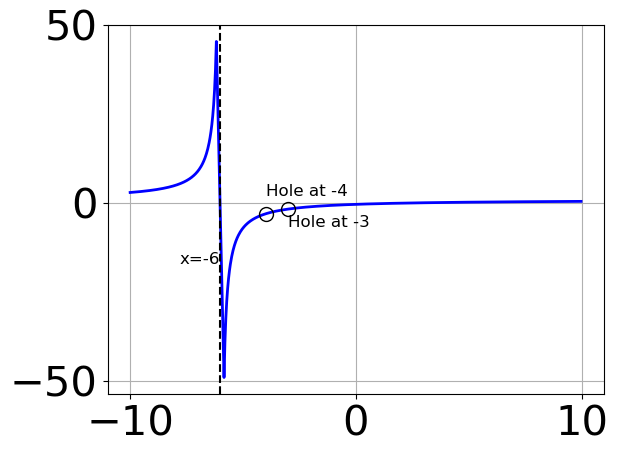
\includegraphics[width=0.5\textwidth]{../Figures/identifyGraphOfRationalFunctionCopyC.png}
\end{center}
\begin{enumerate}[label=\Alph*.]
\item \( f(x)=\frac{x^{3} +5.0 x^{2} -2.0 x -24.0}{x^{3} +13.0 x^{2} +54.0 x + 72.0} \)
\item \( f(x)=\frac{x^{3} -1.0 x^{2} -16.0 x -20.0}{x^{3} -13.0 x^{2} +54.0 x -72.0} \)
\item \( f(x)=\frac{x^{3} -1.0 x^{2} -22.0 x + 40.0}{x^{3} +13.0 x^{2} +54.0 x + 72.0} \)
\item \( f(x)=\frac{x^{3} -5.0 x^{2} -2.0 x + 24.0}{x^{3} -13.0 x^{2} +54.0 x -72.0} \)
\item \( \text{None of the above are possible equations for the graph.} \)

\end{enumerate} }
\litem{
Determine the horizontal and/or oblique asymptotes in the rational function below.\[ f(x) = \frac{20x^{3} -47 x^{2} -54 x + 45}{-20x^{3} +14 x^{2} -18} \]\begin{enumerate}[label=\Alph*.]
\item \( \text{Vertical Asymptote of } y = 3  \)
\item \( \text{Vertical Asymptote of } y = -0.500  \)
\item \( \text{None of the above} \)
\item \( \text{Horizontal Asymptote of } y = 0  \)
\item \( \text{Horizontal Asymptote of } y = -1.000  \)

\end{enumerate} }
\litem{
Which of the following functions \textit{could} be the graph below?
\begin{center}
    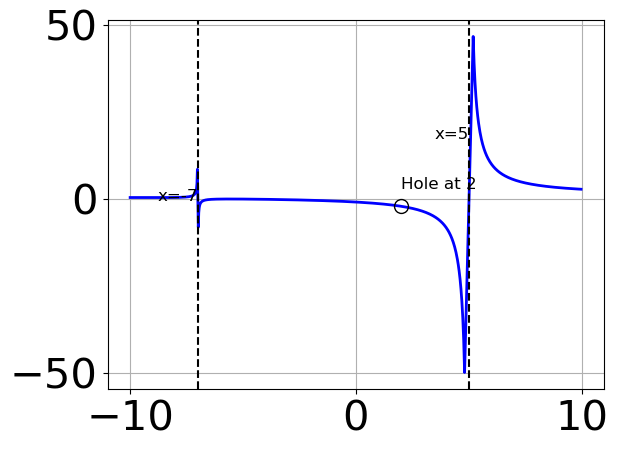
\includegraphics[width=0.5\textwidth]{../Figures/identifyGraphOfRationalFunctionC.png}
\end{center}
\begin{enumerate}[label=\Alph*.]
\item \( f(x)=\frac{x^{3} -5.0 x^{2} -36.0 x + 180.0}{x^{3} -39.0 x -70.0} \)
\item \( f(x)=\frac{x^{3} +13.0 x^{2} +52.0 x + 60.0}{x^{3} -39.0 x + 70.0} \)
\item \( f(x)=\frac{x^{3} +9.0 x^{2} +8.0 x -60.0}{x^{3} -39.0 x + 70.0} \)
\item \( f(x)=\frac{x^{3} -9.0 x^{2} +8.0 x + 60.0}{x^{3} -39.0 x -70.0} \)
\item \( \text{None of the above are possible equations for the graph.} \)

\end{enumerate} }
\litem{
Determine the vertical asymptotes and holes in the rational function below.\[ f(x) = \frac{9x^{3} -9 x^{2} -88 x -80}{9x^{2} +9 x -10} \]\begin{enumerate}[label=\Alph*.]
\item \( \text{Vertical Asymptotes of } x = 0.667 \text{ and } x = -1.333 \text{ with a hole at } x = -1.667 \)
\item \( \text{Vertical Asymptote of } x = 0.667 \text{ and hole at } x = -1.667 \)
\item \( \text{Vertical Asymptote of } x = 1.0 \text{ and hole at } x = -1.667 \)
\item \( \text{Vertical Asymptotes of } x = 0.667 \text{ and } x = -1.667 \text{ with no holes.} \)
\item \( \text{Holes at } x = 0.667 \text{ and } x = -1.667 \text{ with no vertical asymptotes.} \)

\end{enumerate} }
\litem{
Determine the horizontal and/or oblique asymptotes in the rational function below.\[ f(x) = \frac{10x^{3} -13 x^{2} -46 x + 40}{-10x^{3} +46 x^{2} +52 x + 20} \]\begin{enumerate}[label=\Alph*.]
\item \( \text{Vertical Asymptote of } y = -0.400  \)
\item \( \text{Vertical Asymptote of } y = -2  \)
\item \( \text{Horizontal Asymptote of } y = -1.000  \)
\item \( \text{Horizontal Asymptote of } y = 0  \)
\item \( \text{None of the above} \)

\end{enumerate} }
\litem{
Determine the vertical asymptotes and holes in the rational function below.\[ f(x) = \frac{12x^{3} -17 x^{2} -104 x -80}{9x^{2} +6 x -8} \]\begin{enumerate}[label=\Alph*.]
\item \( \text{Vertical Asymptotes of } x = 0.667 \text{ and } x = -1.25 \text{ with a hole at } x = -1.333 \)
\item \( \text{Holes at } x = 0.667 \text{ and } x = -1.333 \text{ with no vertical asymptotes.} \)
\item \( \text{Vertical Asymptotes of } x = 0.667 \text{ and } x = -1.333 \text{ with no holes.} \)
\item \( \text{Vertical Asymptote of } x = 1.333 \text{ and hole at } x = -1.333 \)
\item \( \text{Vertical Asymptote of } x = 0.667 \text{ and hole at } x = -1.333 \)

\end{enumerate} }
\litem{
Determine the horizontal and/or oblique asymptotes in the rational function below.\[ f(x) = \frac{6x^{3} -49 x^{2} +125 x -100}{2x^{2} +3 x -20} \]\begin{enumerate}[label=\Alph*.]
\item \( \text{Horizontal Asymptote at } y = -4.0 \)
\item \( \text{Horizontal Asymptote of } y = 3.0  \)
\item \( \text{Oblique Asymptote of } y = 3x -29. \)
\item \( \text{Horizontal Asymptote of } y = 3.0 \text{ and Oblique Asymptote of } y = 3x -29 \)
\item \( \text{Horizontal Asymptote of } y = -4.0 \text{ and Oblique Asymptote of } y = 3x -29 \)

\end{enumerate} }
\litem{
Determine the horizontal and/or oblique asymptotes in the rational function below.\[ f(x) = \frac{12x^{3} -29 x^{2} +23 x -6}{3x^{2} +10 x -8} \]\begin{enumerate}[label=\Alph*.]
\item \( \text{Horizontal Asymptote of } y = 4.0 \text{ and Oblique Asymptote of } y = 4x -23 \)
\item \( \text{Horizontal Asymptote of } y = -4.0 \text{ and Oblique Asymptote of } y = 4x -23 \)
\item \( \text{Horizontal Asymptote of } y = 4.0  \)
\item \( \text{Horizontal Asymptote at } y = -4.0 \)
\item \( \text{Oblique Asymptote of } y = 4x -23. \)

\end{enumerate} }
\end{enumerate}

\end{document}